\documentclass{book}
\usepackage{xeCJK}
\usepackage{graphicx} % Required for inserting images
\usepackage{ulem} % underline
\usepackage{amsmath,amssymb,amsthm}
\theoremstyle{definition}
\newtheorem{definition}{Definition}[section]
\newtheorem{theorem}{Theorem}[section]
\newtheorem{remark}{Remark}[section]
\newtheorem{proposition}{Proposition}[section]

\usepackage{indentfirst} 
\setlength{\parindent}{2em}

\title{Lecture notes of Analysis}
\author{Penggao Yan}
\date{October 2023}

\begin{document}

\maketitle


\chapter{Introduction}
\section{Lecture 1}
\begin{itemize}
    \item P1. 导论 
    \item Create Date: 26 Oct. 2023
    \item Last Update: 7 Nov. 2023
\end{itemize}

\chapter{L1-L10}
\section{Lecture 2}
\begin{itemize}
    \item P2. 最小上界、最大下界、Dedekind cut、数列极限的定义与性质 
    \item Create Date: 26 Oct. 2023
    \item Last Update: 27 Oct. 2023
\end{itemize}

\subsection{最小上界、最大下界、Dedekind cut}
\label{subsec:minmaxbound}
\begin{definition}[Upper bound and lower bound]
Let $\mathcal{S} \subseteq \mathbb{R}$ and $r \in \mathbb{R}$, we say that:
\begin{enumerate}
    \item $r$ is an upper (resp. lower) bound of $\mathcal{S}$ if 
    \begin{equation}
        \forall s \in \mathcal{S}, r \ge s 
        ~\text{(resp. } \forall s \in \mathcal{S}, r \le s \text{)} \,.
    \end{equation}
   
    \item $r$ is the greatest (resp. least) element of $\mathcal{S}$ if 
    \begin{enumerate}
        \item $r$ is an upper (resp. lower) bound of $\mathcal{S}$; and 
        \item $r\in\mathcal{S}$.
    \end{enumerate}
    We can use the notation: 
    \begin{equation}
        r=\max \mathcal{S}
        ~\text{(resp. } r=\min \mathcal{S} \text{)}  \,.
    \end{equation}

    \item $r$ is the least upper (greatest lower) bound of $\mathcal{S}$ if 
    \begin{equation}
    \begin{aligned}
        r=&\min \left\{ u\in\mathbb{R} | u \text{ is an upper bound of } \mathcal{S} \right\} \\
        \text{(resp. } r=&\max \left\{ u\in\mathbb{R} | u \text{ is a lower bound of } \mathcal{S}  \right\} \text{)} \,.
    \end{aligned}
    \end{equation}
    We can use the notation: 
    \begin{equation}
        r=\sup \mathcal{S}
        ~\text{(resp. } r=\inf \mathcal{S} \text{)}  \,.
    \end{equation}
\end{enumerate}
\end{definition}

\noindent \textbf{Exe 0}: 自己举例,任选一个集合$\mathcal{S}$ ,判断它是否有上下界,如果有分别是多少。\\
~\\
在least upper (or greatest lower) bound,我们最常用到的定理是什么? 
\begin{itemize}
    \item ``比least upper bound小的不是upper bound, 比 greatest lower bound 大的不是lower bound". 这可以作为脑子里的一个反证工作。
    \item Every $r\in\mathbb{R}$ is an upper and lower bound of $\emptyset$. 我们可以从定义出发来想这件事,因此,我们一般不会谈论空集的上下界。
\end{itemize}
对于第二点,我们有如下 \textbf{convention}: \\
\begin{enumerate}
    \item We write 
    \begin{equation}
        \sup \mathcal{S}=\infty
        ~\text{(resp. } \inf \mathcal{S} =-\infty \text{)}  \,,
    \end{equation}
    if and only if (iif.) $\mathcal{S}$ has no upper (resp. lower) bound. If this is the case, we say that $\sup \mathcal{S}$ (resp. $\inf \mathcal{S}$) doesn't exist.
    \item $\mathcal{S}$ is bounded from above (resp. below) iff. $\mathcal{S}$ has an upper (resp. lower) bound.
\end{enumerate}

\begin{definition}[Dedekind cut]
Let $\mathcal{A}, \mathcal{B} \subseteq \mathbb{R}$. We say that $(\mathcal{A}, \mathcal{B})$ is Dedekind cut (of $\mathbb{R}$) if
\begin{enumerate}
    \item $\mathcal{A} \neq \emptyset \neq \mathcal{B}$, and
    \item $\mathcal{A} \cup \mathcal{B} = \mathbb{R}$, and
    \item $\forall a \in \mathcal{A}, b \in \mathcal{B}~[a<b]$.
\end{enumerate}
We usually call $\mathcal{A}$ (resp. $\mathcal{B}$)  the lower (resp. upper) part of $(\mathcal{A}, \mathcal{B})$ .
\end{definition}

From now on (until Dr. Qi say stop), we assume that $\mathbb{R}$ has the following property: \\
~\\
(\textbf{Dedekind's gapless property}) If $(\mathcal{A}, \mathcal{B})$ is a D-cut of $\mathbb{R}$ , then exactly one of the following happens:
\begin{enumerate}
    \item $\max \mathcal{A}$ exists but $\min \mathcal{B}$ doesn't 
    \item  $\min \mathcal{B}$  exists but $\max \mathcal{A}$ doesn't 
\end{enumerate}
We call $\max \mathcal{A}$ in (1) (resp. $\min \mathcal{B}$) is the cutting of $(\mathcal{A}, \mathcal{B})$.\\
~\\
\textbf{Exe 1}: We may define Dedekind cuts of $\mathbb{Q}$ (or $\mathbb{Z}$) similarly. Does the Dedekind gapless property still hold for $\mathbb{Q}$ (or $\mathbb{Z}$)?\\
\textbf{Hint}: Consider $\mathcal{B}=\left\{ x \in \mathbb{Q} | x>0, x^2>2 \right\}$. You are allowed to use the fact $\forall r \in \mathbb{Q} [r\neq2]$.\\
\textbf{Hint}: 假设$b$是$\mathcal{B}$的最小数,我们需要在$\mathcal{B}$ 里面找一个比$b$更小的数.

\begin{theorem}[Weierstrass]
Let $\emptyset\neq\mathcal{S}\subseteq\mathbb{R}$ . If $\mathcal{S}$ has an upper bound, then $\sup \mathcal{S}$ exists.
\end{theorem}
\begin{proof}
Let $\mathcal{B}=\{b\in\mathbb{R} | b~\text{is an upper bound of}~ \mathcal{S}\}$ and $\mathcal{A}=\mathbb{R}\setminus\mathcal{B}$. It is sensed that $(\mathcal{A}, \mathcal{B})$ is a D-cut of $\mathbb{R}$ .\\
\textbf{Goal}: We need to show that $\min \mathcal{B}$ exists.\\
\textbf{Step 1}:  Prove $(\mathcal{A}, \mathcal{B})$ is a D-cut of $\mathbb{R}$. Our thoughts are:
\begin{enumerate}
    \item $\mathcal{S}$ has upper bound $\Rightarrow$ $\mathcal{S}\neq\emptyset$ $\Rightarrow$ $\mathcal{A}\neq\emptyset$.
    \item $\mathcal{S}$ has upper bound $\Leftrightarrow$$\mathcal{B}\neq\emptyset$.
    \item $\mathcal{A}=\mathbb{R}\setminus\mathcal{B}$ $\Rightarrow$ $\mathcal{A}\cup\mathcal{B}=\mathbb{R}$.
    \item For $a\in \mathcal{A}$ and $b\in\mathcal{B}$ , we need to show that $a<b$. Were this false, then $a\geq b$ , and hence $a$ is a upper bound of $\mathcal{S}$, i.e., $a\in\mathcal{B}$. This is impossible. Therefore, $a<b$.
\end{enumerate}
It is proved that $(\mathcal{A}, \mathcal{B})$ is a D-cut of $\mathbb{R}$.\\
\textbf{Step 2}: Prove $\min \mathcal{B}$ exists. Our thoughts are:
\begin{enumerate}
    \item Were this false, according to Dedekind's gapless property, $\max A$ exists, denoted by $a_0$. We have
    \begin{equation}
    \begin{aligned}
        a_0\in \mathcal{A} \Leftrightarrow & a_0 \not\in \mathcal{B} \\
                            \Leftrightarrow & a_0~\text{is not an upper bound of}~\mathcal{S} \,.\\
    \end{aligned}
    \end{equation}
    This means at least one element in $\mathcal{S}$ is larger than $a_0$, i.e.,
    \begin{equation}
        \Leftrightarrow \exists s_0 \in \mathcal{S}~[a_0 < s_0] \,.
    \end{equation}
    \item Since $a_0 < s_0$, $s_0$ cannot belong to $\mathcal{A}$,i.e.
    \begin{equation}
        \Leftrightarrow s_0 \not\in \mathcal{A} \Leftrightarrow s_0 \in \mathcal{B} \,.
    \end{equation}
    \item Choose $x$ such that $a_0<x<s_0$ (We can always find a $x$ that satisfies this equation,e.g., $x=(a_0+s_0)/2$). In this case, $x\in \mathcal{B} \Leftrightarrow x~\text{is an upper bound of}~ \mathcal{S}$ . However, $s_0 \in \mathcal{S}$. This is impossible. 
\end{enumerate}
Therefore, $\min \mathcal{B}$ exists.\\
\end{proof}

\noindent \textbf{Exe 2}. Prove the following statement:\\
(\textbf{The Archimedean property}) $\forall r\in\mathbb{R}~\left[r>0\Rightarrow \exists n\in\mathbb{N}~\left[1/n<r\right]\right]$.\\
直观理解:将整数$1$切为$n$ 等分,当$n$最够大的时候,每一份将比任意正实数小.\\
\textbf{Hint}: Rephrase this statement in a way linking it to the upper bounds of the set $\mathcal{S}=\mathbb{N}\subseteq\mathbb{R}$. You can consider to prove whether an positive integer has an upper bound in $\mathbb{R}$.

\subsection{数列极限的定义与性质}

\begin{definition}[Limit]
\label{def:limit}
Let $a_n~(n\in\mathbb{N})$ (or say $\left\{ a_n \right\}_{n=1}^{n}$) be a sequence in $\mathbb{R}$ and $L\in\mathbb{R}$. We say that $a_n$ converges to $L$ (as $n\rightarrow\infty$) if
\begin{equation}
    \forall \epsilon>0~ \exists N\in \mathbb{N} ~[n\ge N \mathbb \Rightarrow |a_n-L|<\epsilon] \,.
\end{equation}
This means that 第N项后所有的项都要落在Fig.\ref{fig:limit}红色区间内.\\
~\\
\uline{Terminology}. If such $L$ exists (resp. doesn't exist), we call it the limit of $a_n$ and call $a_n$ is a convergent (resp. divergent )sequence. We can use the notation:
\begin{equation}
    \lim_{n\rightarrow \infty} a_n = L \,.
\end{equation}
\uline{Some generalized notations}. 
\begin{equation}
\begin{aligned}
\lim_{n\to \infty} a_n = \infty \Rightarrow & \forall M>0~ \exists N\in \mathbb{N} ~[n\ge N \mathbb \Rightarrow a_n\ge M]\\
\lim_{n\to \infty} a_n = -\infty \Rightarrow & \forall M>0~ \exists N\in \mathbb{N} ~[n\ge N \mathbb \Rightarrow a_n\le M] \,.
\end{aligned}
\end{equation}
In these two cases, we don't say that $a_n$ is convergent.
\end{definition}

\begin{figure}
    \centering
    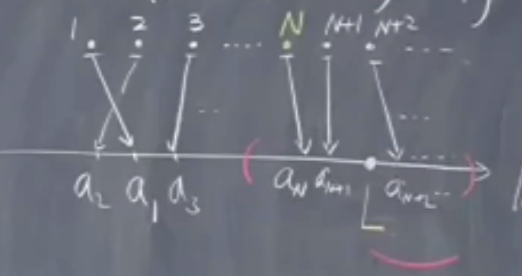
\includegraphics[width=0.5\linewidth]{image.png}
    \caption{Enter Caption}
    \label{fig:limit}
\end{figure}

\noindent \textbf{Exe 3}. 
\begin{enumerate}
    \item Prove that $lim_{n\to\infty} a_n = L ~ lim_{n\to\infty} a_n = M \Rightarrow L=M$.\\
    \textbf{Hint}. 分别在L和M处取一个小区间,让他们不相交,根据极限定义来证明 (反证)。
    \item Prove that $a_n (n\in\mathbb{N})$ is convergent $\Rightarrow$ $\left\{ a_n | n\in \mathbb{N} \right\}$ is bounded.\\
    \textbf{Hint}. $a_n$ 收敛说明某项(例如10,000 项)后,所有项都被包在某个区间内,这说明10,000 项后所有项都是有界的。我们只需要再证明10,000之前的所有项也是有界的即可。\\
    \item Prove that if $a_n\le b_n$ for all $n\in\mathbb{N}$, $\lim_{n\to \infty} a_n=L$ and  $\lim_{n\to \infty} b_n=M$, then $L\le M$. What if $\leq$ is replaced by $<$?
\end{enumerate}

\begin{remark}
Changing of removing finitely many terms in $a_n$ does not affect $a_n (n\in\mathbb{N})$'s being convergent (and its limit)/divergent. 
\end{remark}
\begin{proposition}
\label{propo:Arithmetic}
If $\lim_{n\to \infty} a_n = L$ and $\lim_{n\to \infty} b_n =M$, then 
\begin{enumerate}
    \item $\lim_{n\to \infty} a_n \pm b_n = L\pm M $
    \item $\lim_{n\to \infty} a_n b_n = LM $
    \item if $M\neq0$, then $b_n \neq 0$ for all but finitely many $n$, and $\lim_{n\to \infty} a_n/b_n = L/M $ (Hint: we can remove the terms with $b_n=0$; removing finitely many terms in $b_n$ does not affect $b_n$'s limit).
\end{enumerate}
\end{proposition}
\begin{proof}
(1) Consider $\left| (a_n \pm b_n) - (L\pm M) \right|$, we have 
\begin{equation}
\begin{aligned}
    \left| (a_n \pm b_n) - (L\pm M) \right| {=}& \left| (a_n - L) \pm (b_n- M) \right| \\
                                          {\leq}& \left| a_n - L\right| + \left| b_n - M\right|
\end{aligned}
\end{equation}
\begin{equation}
\begin{aligned}
    \forall \epsilon>0~\exists N_1, N_2 \in \mathbb{N}~&[n \geq N_1 \Rightarrow |a_n-L|<\epsilon/2]\\
    \text{and}~&[n\geq N_2 \Rightarrow |b_n-M|<\epsilon/2] \,.
\end{aligned}
\end{equation}
Let $N=\max\left\{N_1, N_2\right\}$. Then $n \geq N \Rightarrow \left| a_n - L\right| + \left| b_n - M\right| < \epsilon/2+\epsilon/2=\epsilon$.\\
Therefore, $\forall \epsilon>0 ~ \left| (a_n \pm b_n) - (L\pm M) \right|<\epsilon$. \\
~\\
\noindent (2) Consider $\left| a_n b_n - LM \right|$, we have
\begin{equation}
    \begin{aligned}
        \left| a_n b_n - LM \right|{=}& \left| a_n b_n -L b_n + L b_n LM \right|\\
                                   {=}& \left| (a_n - L) b_n + L(b_n - M)\right|\\
                                   {\leq}& \left| a_n-L\right||b_n|+|L||b_n-M| \,.
    \end{aligned}
\end{equation}
Choose $C>0$ such that $|b_n| \leq C$ and $|L|\leq C$ for all $n\in \mathbb{N}$ (PS: $|b_n| \leq C$ 的存在性可以用Ex.3(2)证明). Then we have
\begin{equation}
        \left| a_n-L\right||b_n|+|L|\left|b_n-M\right| \leq C\left|a_n-L \right| + C\left|b_n-M\right| \,.
\end{equation}
\begin{flushright}(三角不等式)\end{flushright}
\begin{equation}
    \forall \epsilon>0~\exists N\in \mathbb{N} \left[ n\geq\mathbb{N} \Rightarrow \left|a_n-L\right|<\frac{\epsilon}{2C}~\text{and}~ \left|b_n-M\right|<\frac{\epsilon}{2C} \right] \,.
\end{equation}
Therefore,
\begin{equation}
    \left| a_n b_n - LM \right|<C\times\frac{\epsilon}{2C}+C\times\frac{\epsilon}{2C}=\epsilon \,.
\end{equation}
\end{proof}
\noindent\textbf{Exe 4}. 
\begin{enumerate}
    \item Prove (3) of  Proposition \ref{propo:Arithmetic}. \\
\textbf{Hint}: $a_n/b_n = L/M $ can be written as $a_n \frac{1}{n_n} = L \frac{1}{M}$. You only need to prove $\lim_{n\to \infty} \frac{1}{b_n} = \frac{1}{M}$ when $\lim_{n\to \infty} a_n/b_n = L/M $. Nevertheless, you are wellcome to prove this Proposition following the above process.
\item (Optional) What if $L=\pm \infty$  or  $M=\pm \infty$  in  Proposition \ref{propo:Arithmetic}. \\
    \item If $a_n=\frac{1-(\frac{1}{2})^n}{1-\frac{1}{2}}$, prove that  $\lim_{n\to \infty} a_n = \frac{1}{1-\frac{1}{2}}$. You can use knowledge learned so far. \\
    \textbf{Hint}: 阿基米德性质.
\end{enumerate}

\section{Lecture 3}
\begin{itemize}
    \item P3. 單調數列的收斂性、區間套定理、Cauchy 數列的概念 
    \item Create Date: 7 Nov. 2023
    \item Last Update: 7 Nov. 2023
\end{itemize}
\subsection{單調數列的收斂性}
\noindent\textbf{Example} If a>1, then $\lim_{n \to \infty} \frac{1}{a^n}=0$.
\begin{equation}
    \frac{1}{a^n}=\frac{1}{\left(1+\left(a-1\right)\right)^n}
\end{equation}
Let $b=a-1>0$, 利用二项式定理展开分母可得,
\begin{equation}
\begin{aligned}
    \left(1+b\right)^n {\geq}& 1+nb\\
    \lim_{n \to \infty} \frac{1}{a^n} {\leq}& \lim_{n \to \infty}\frac{1}{1+nb}=0\,.
\end{aligned}
\end{equation}
Since $\frac{1}{a^n}\geq 0$, we have $\lim_{n \to \infty} \frac{1}{a^n}=0$.\\
~\\
\noindent \textbf{Exe 1}(Squzzing therome). If $a_n\leq c_n \leq b_n~n\in\mathbb{N}$, $\lim_{n \to \infty} a_n=L$ and $\lim_{n \to \infty} b_n=L$, prove that $\lim_{n \to \infty} c_n=L$.\\
\textbf{Hint}: Use definition of limit.
\begin{definition}[monotone]
    A seq. $a_n~n\in\mathbb{N}$ in $\mathbb{R}$ is 
    \begin{itemize}
        \item nondecreasing monotone/ increasing (resp. nonincreasing monotone/ decreasing)if $\forall n\in\mathbb{N}~ a-N\leq a_{n+1}$ (resp.  $\forall n\in\mathbb{N}~ a-N\geq a_{n+1}$), we use \textbf{notation}:
            \begin{equation}
                a_n \uparrow~\text{(resp.}~a_n \downarrow \text{)}
            \end{equation}
        \item strictly increasing (resp. strictly decreasing) if $\forall n\in\mathbb{N}~ a-N < a_{n+1}$ (resp.  $\forall n\in\mathbb{N}~ a-N > a_{n+1}$), we use \textbf{notation}: 
            \begin{equation}
                a_n \uparrow\uparrow~\text{(resp.}~a_n \downarrow\downarrow \text{)}
            \end{equation}
    \end{itemize}
\end{definition}

\begin{theorem}[??]
   If $a_n\uparrow$ and $\left\{a_n | n\in\mathbb{N}\right\}$ has a upper bound, then $a_n$ converges (to $\sup\left\{ a_n | n \in \mathbb{N}\right\}$).
\end{theorem}
\begin{proof}
Our thinking are:
    \begin{enumerate}
        \item (use the limit property) $\left\{a_n | n\in\mathbb{N}\right\}$ has an upper bound $\Rightarrow$ $L=\sup\left\{ a_n | n\in\mathbb{N} \right\}$ exists. (ref. convention 2 in \ref{subsec:minmaxbound})
        \item (use the monotone property) We claim that $\lim_{n\to\infty} a_n=L$. Now we need to prove it:\\
        $\forall \epsilon~ L-\epsilon<L$ (which means $L-\epsilon$ is not an upper bound) and hence $\exists N\in\mathbb{N}\left[L-\epsilon<a_N \right]$, as shown in Figure \ref{fig:Them2.2.1}. Therefore, we have
        \begin{equation}
            \forall n>N \left[ a_N\leq a_n\right] \,.
        \end{equation}
        Since $a_N>L-\epsilon$ and $a_n\leq L+\epsilon$, we have 
        \begin{equation}
            \left|a_n-L\right|\leq \epsilon \,.
        \end{equation}
        This is the proof of $\forall \epsilon~ L-\epsilon<L$.
    \end{enumerate}
\end{proof}

\begin{figure}
    \centering
    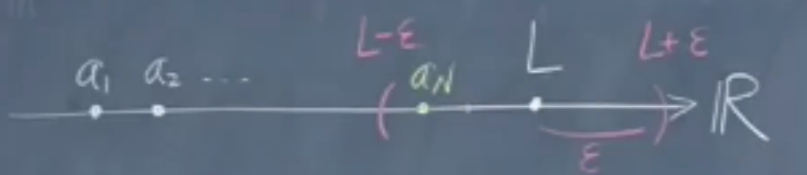
\includegraphics[width=0.7\linewidth]{Them2.2.1.png}
    \caption{Illustrating proof of Them2.2.1.}
    \label{fig:Them2.2.1}
\end{figure}
        
\textbf{Examples}
\begin{enumerate}
    \item A decimal expression (小数表示法) gives a real number: \\
    $0.d_1 d_2 d_3 \dots$
\end{enumerate}




\textbf{update on 0:29:29}


\end{document}

